%\RequirePackage[l2tabu, orthodox]{nag}
\documentclass[hyperref={pdfpagelabels=false}]{beamer}
%\documentclass[handout]{beamer}
\usepackage[ngerman]{babel}
\usepackage{amsmath}
\usepackage{amsfonts}
\usepackage{amssymb}
\usefonttheme{serif}
\usepackage[utf8]{inputenc}
\usepackage {graphicx}
\usepackage [T1]{fontenc}
%\usepackage{listings} %Quellcode mit \lstinline{} oder mit \begin ... darstellen
\usepackage{hyperref}
\usepackage{fancyvrb}

\usepackage{siunitx}
\usepackage{cancel}
\usepackage{slashed}
\usepackage{braket}

\usepackage{animate}
\usepackage{media9}
\usepackage{todonotes}

%\usepackage{caption}
%\usepackage{subcaption}
%\captionsetup[subfigure]{labelformat=empty}

% TikZ
%\usepackage[landscape]{geometry}
%\usepackage{tikz}
%\usetikzlibrary{mindmap}
%\usepackage{metalogo}
%\usepackage{dtklogos}
%\usepackage{adjustbox}

\usepackage{bbding}
\usepackage{overpic}

%\pgfpagesuselayout{4 on 1 with notes}[a4paper,border shrink=5mm]
\title[\LaTeX-Einführung]{Ausgewählite praktische Packages}
\institute{Fachschaft Physik}
\author[Ole, Marco]{Ole Hinrichs, Marco Knipfer}
%\usetheme{Warsaw}
\usetheme{Madrid}
\usecolortheme{default}
\beamertemplatenavigationsymbolsempty
\providecommand{\thispdfpagelabel}[1]{}

\begin{document} 
\begin{frame}{Welche Packages?}
    \begin{block}{}
        \begin{itemize}
            \item todonotes
            \item cancel
            \item braket
            \item microtype
            \item animate
            \item media9 
        \end{itemize}
    \end{block}
\end{frame}
\begin{frame}[fragile]{Das Todonotes Package}
    \begin{block}{Todonotes}
        \begin{itemize}
            \item \verb!\usepackage{todonotes}!
            \item \verb!\todo{}!
            \item \verb!\missingfigure!
            \item \verb!\listoftodos!
        \end{itemize}
    \end{block}
\end{frame}
\begin{frame}[fragile]{Todonotes}
    \begin{center}
        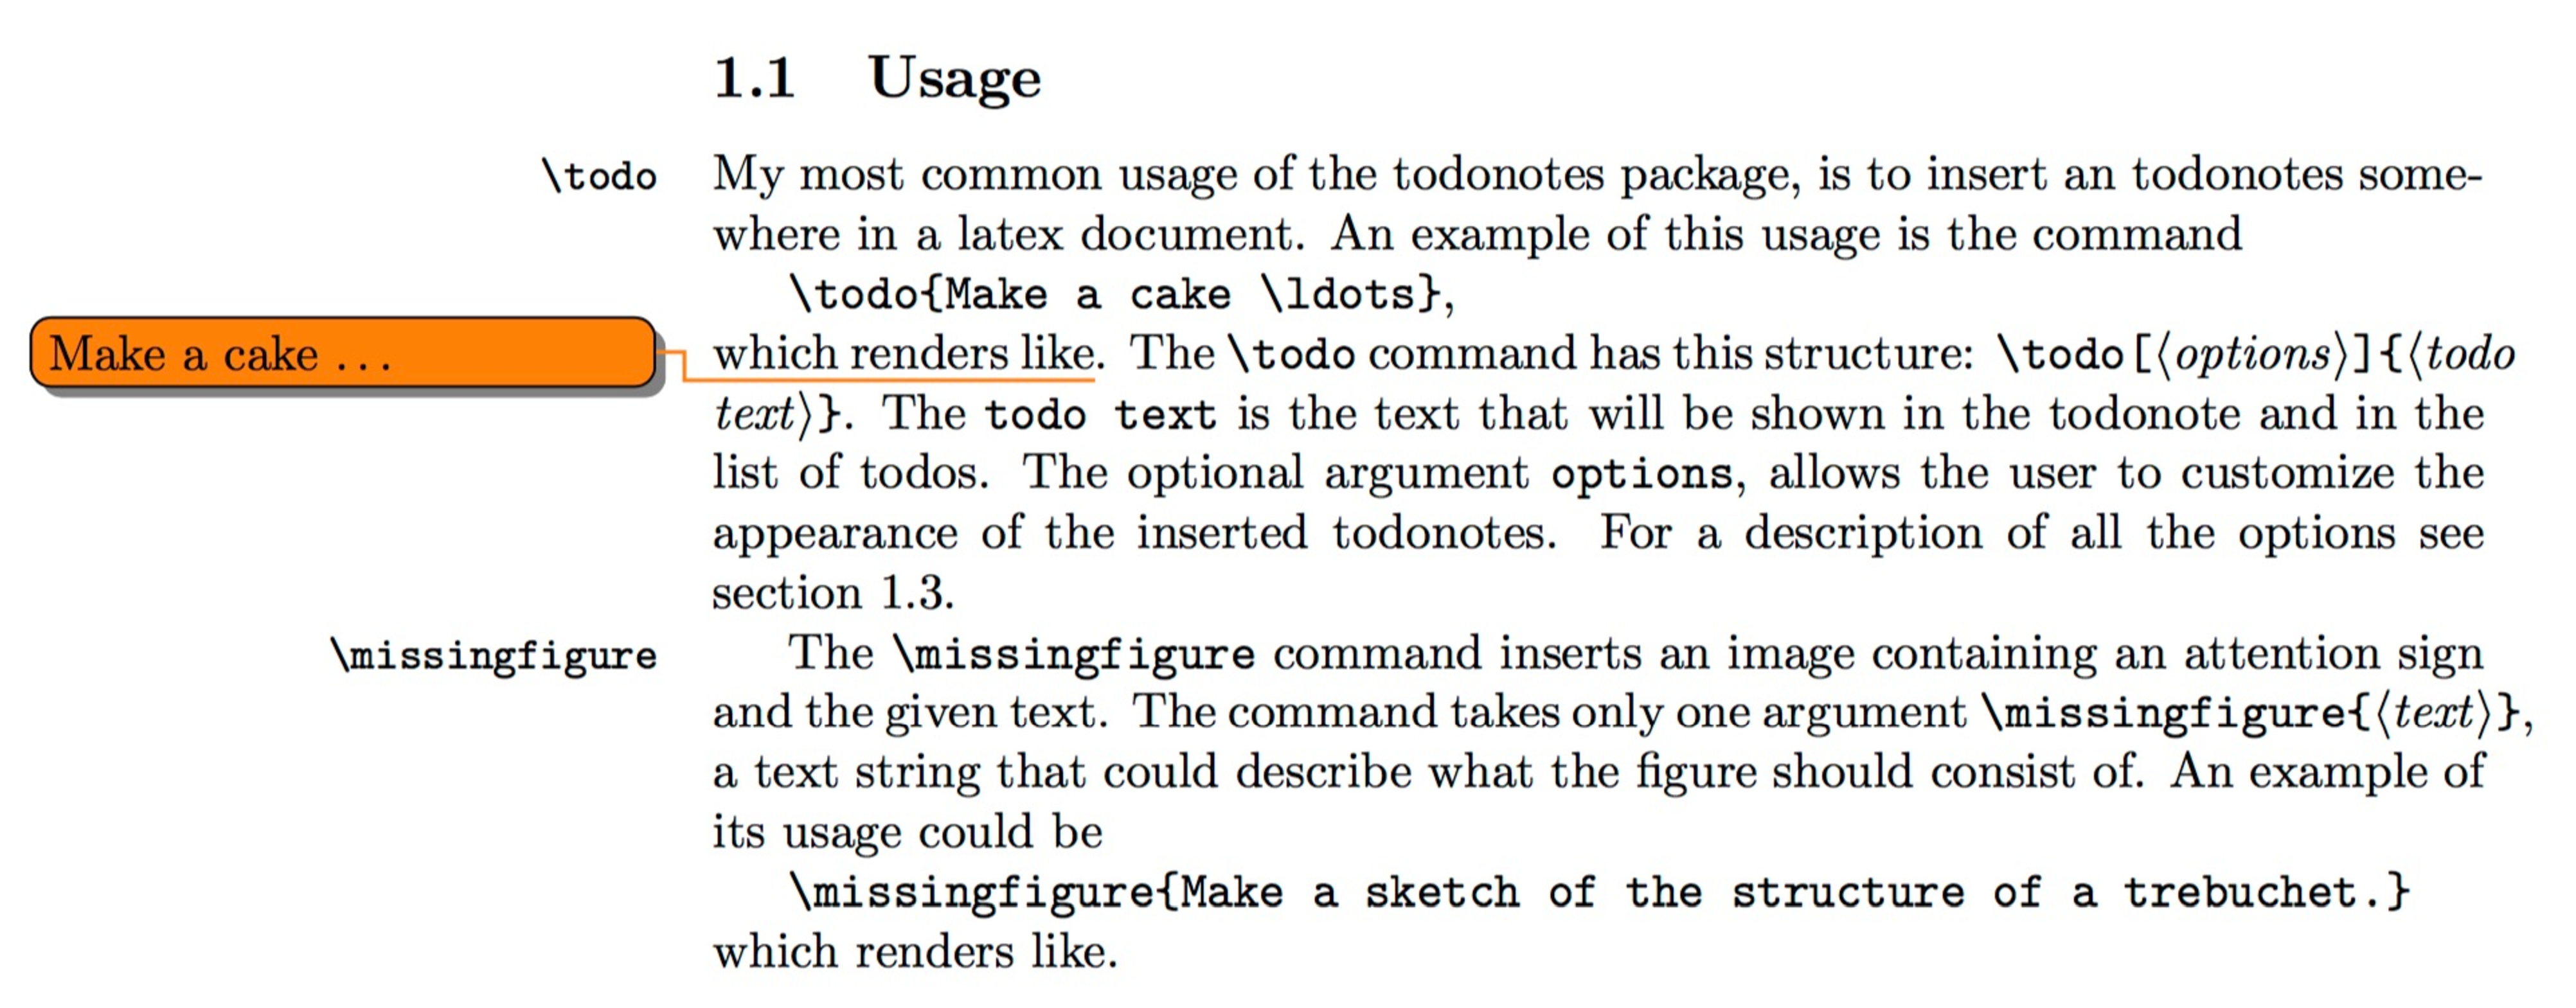
\includegraphics[width = \textwidth]{figures/todo.pdf}
        \newline
    \end{center}
        Aus der Anleitung Todonotes-Anleitung
\end{frame}
\begin{frame}[fragile]{Missingfigure}
    \begin{figure}
        \centering
            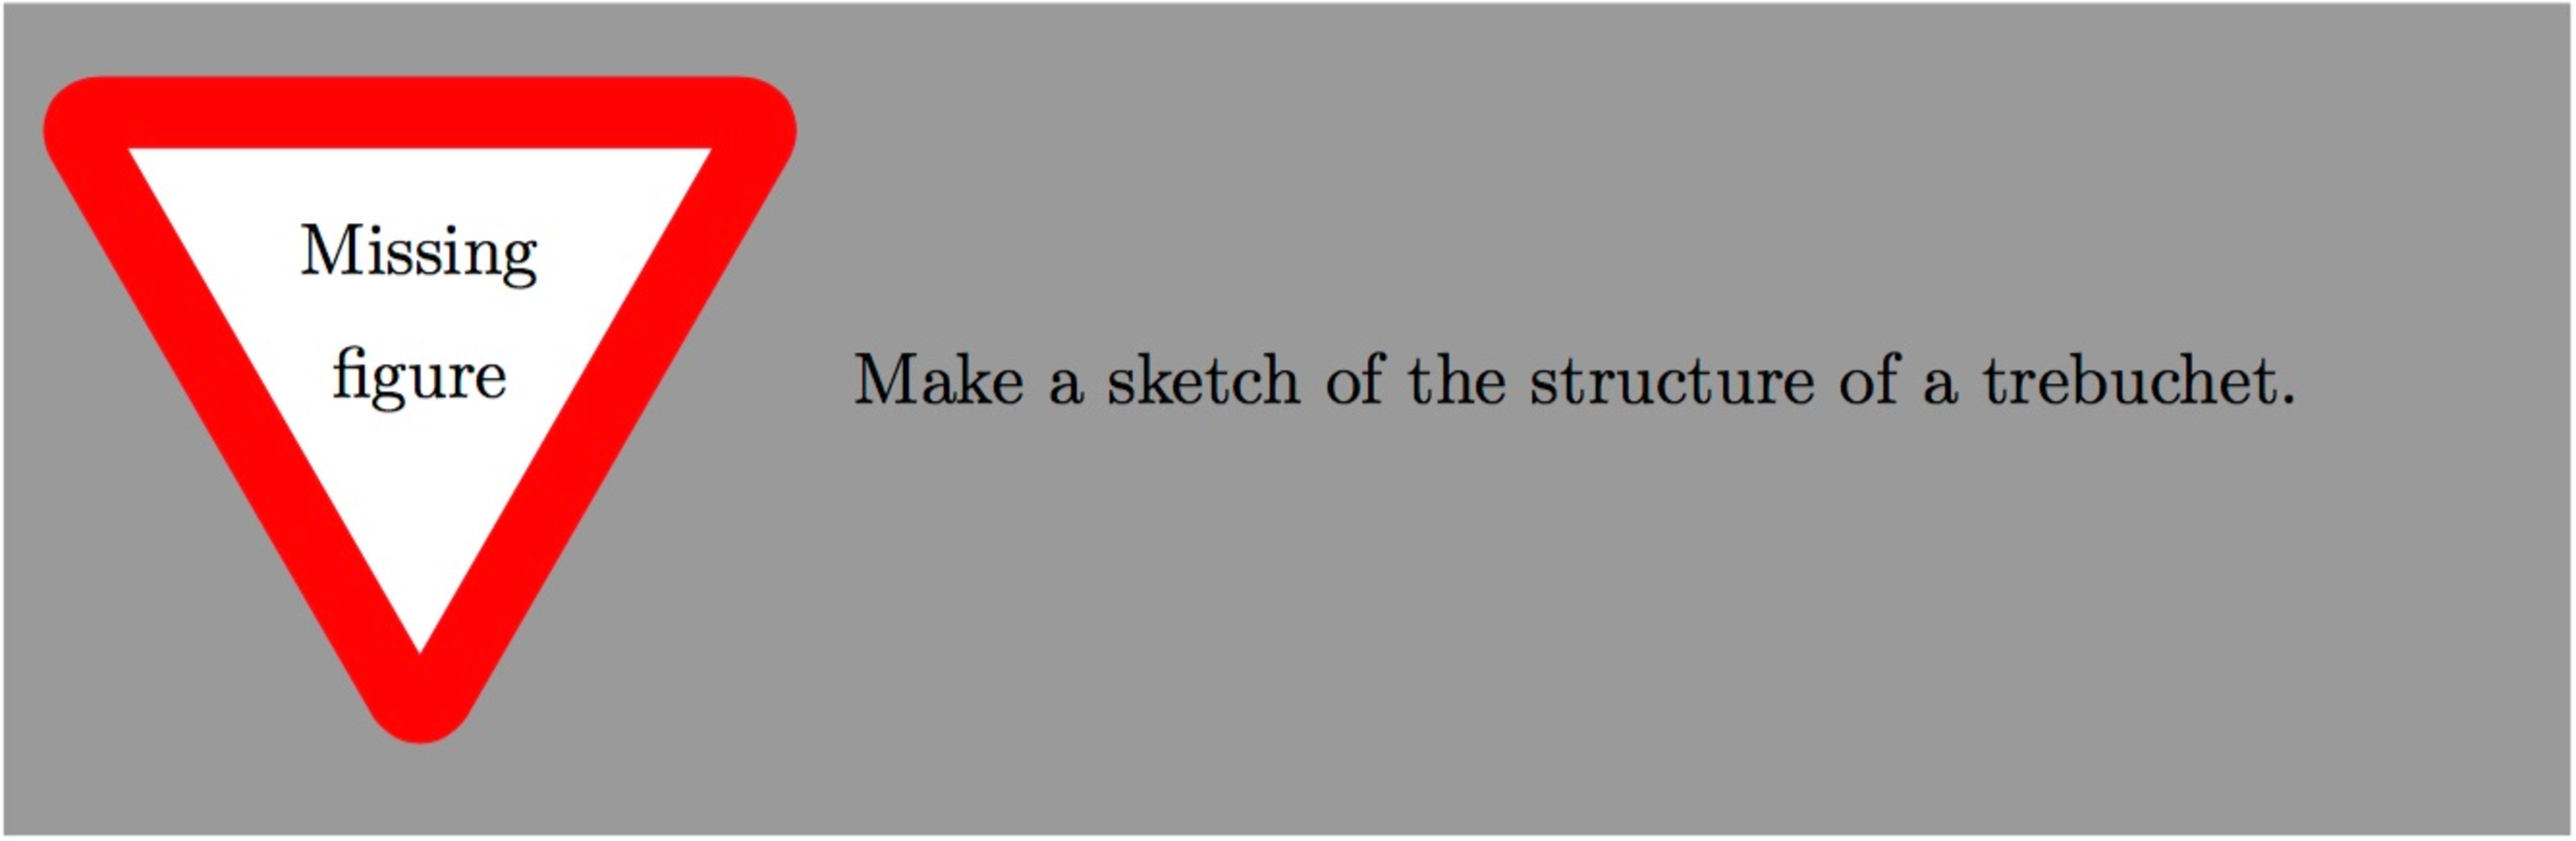
\includegraphics[width = \textwidth]{figures/missingfigure.pdf}
            % wieso geht missingfigure nicht in beamer?
        \caption{Diese Figure fehlt noch}
        \label{fig:missing}
        \begin{Verbatim}
\missingfigure{Make a sketch of the structure of a trebuchet.}
        \end{Verbatim}
    \end{figure}
\end{frame}
\begin{frame}[fragile]{Listoftodos}
    \begin{figure}
        \centering
        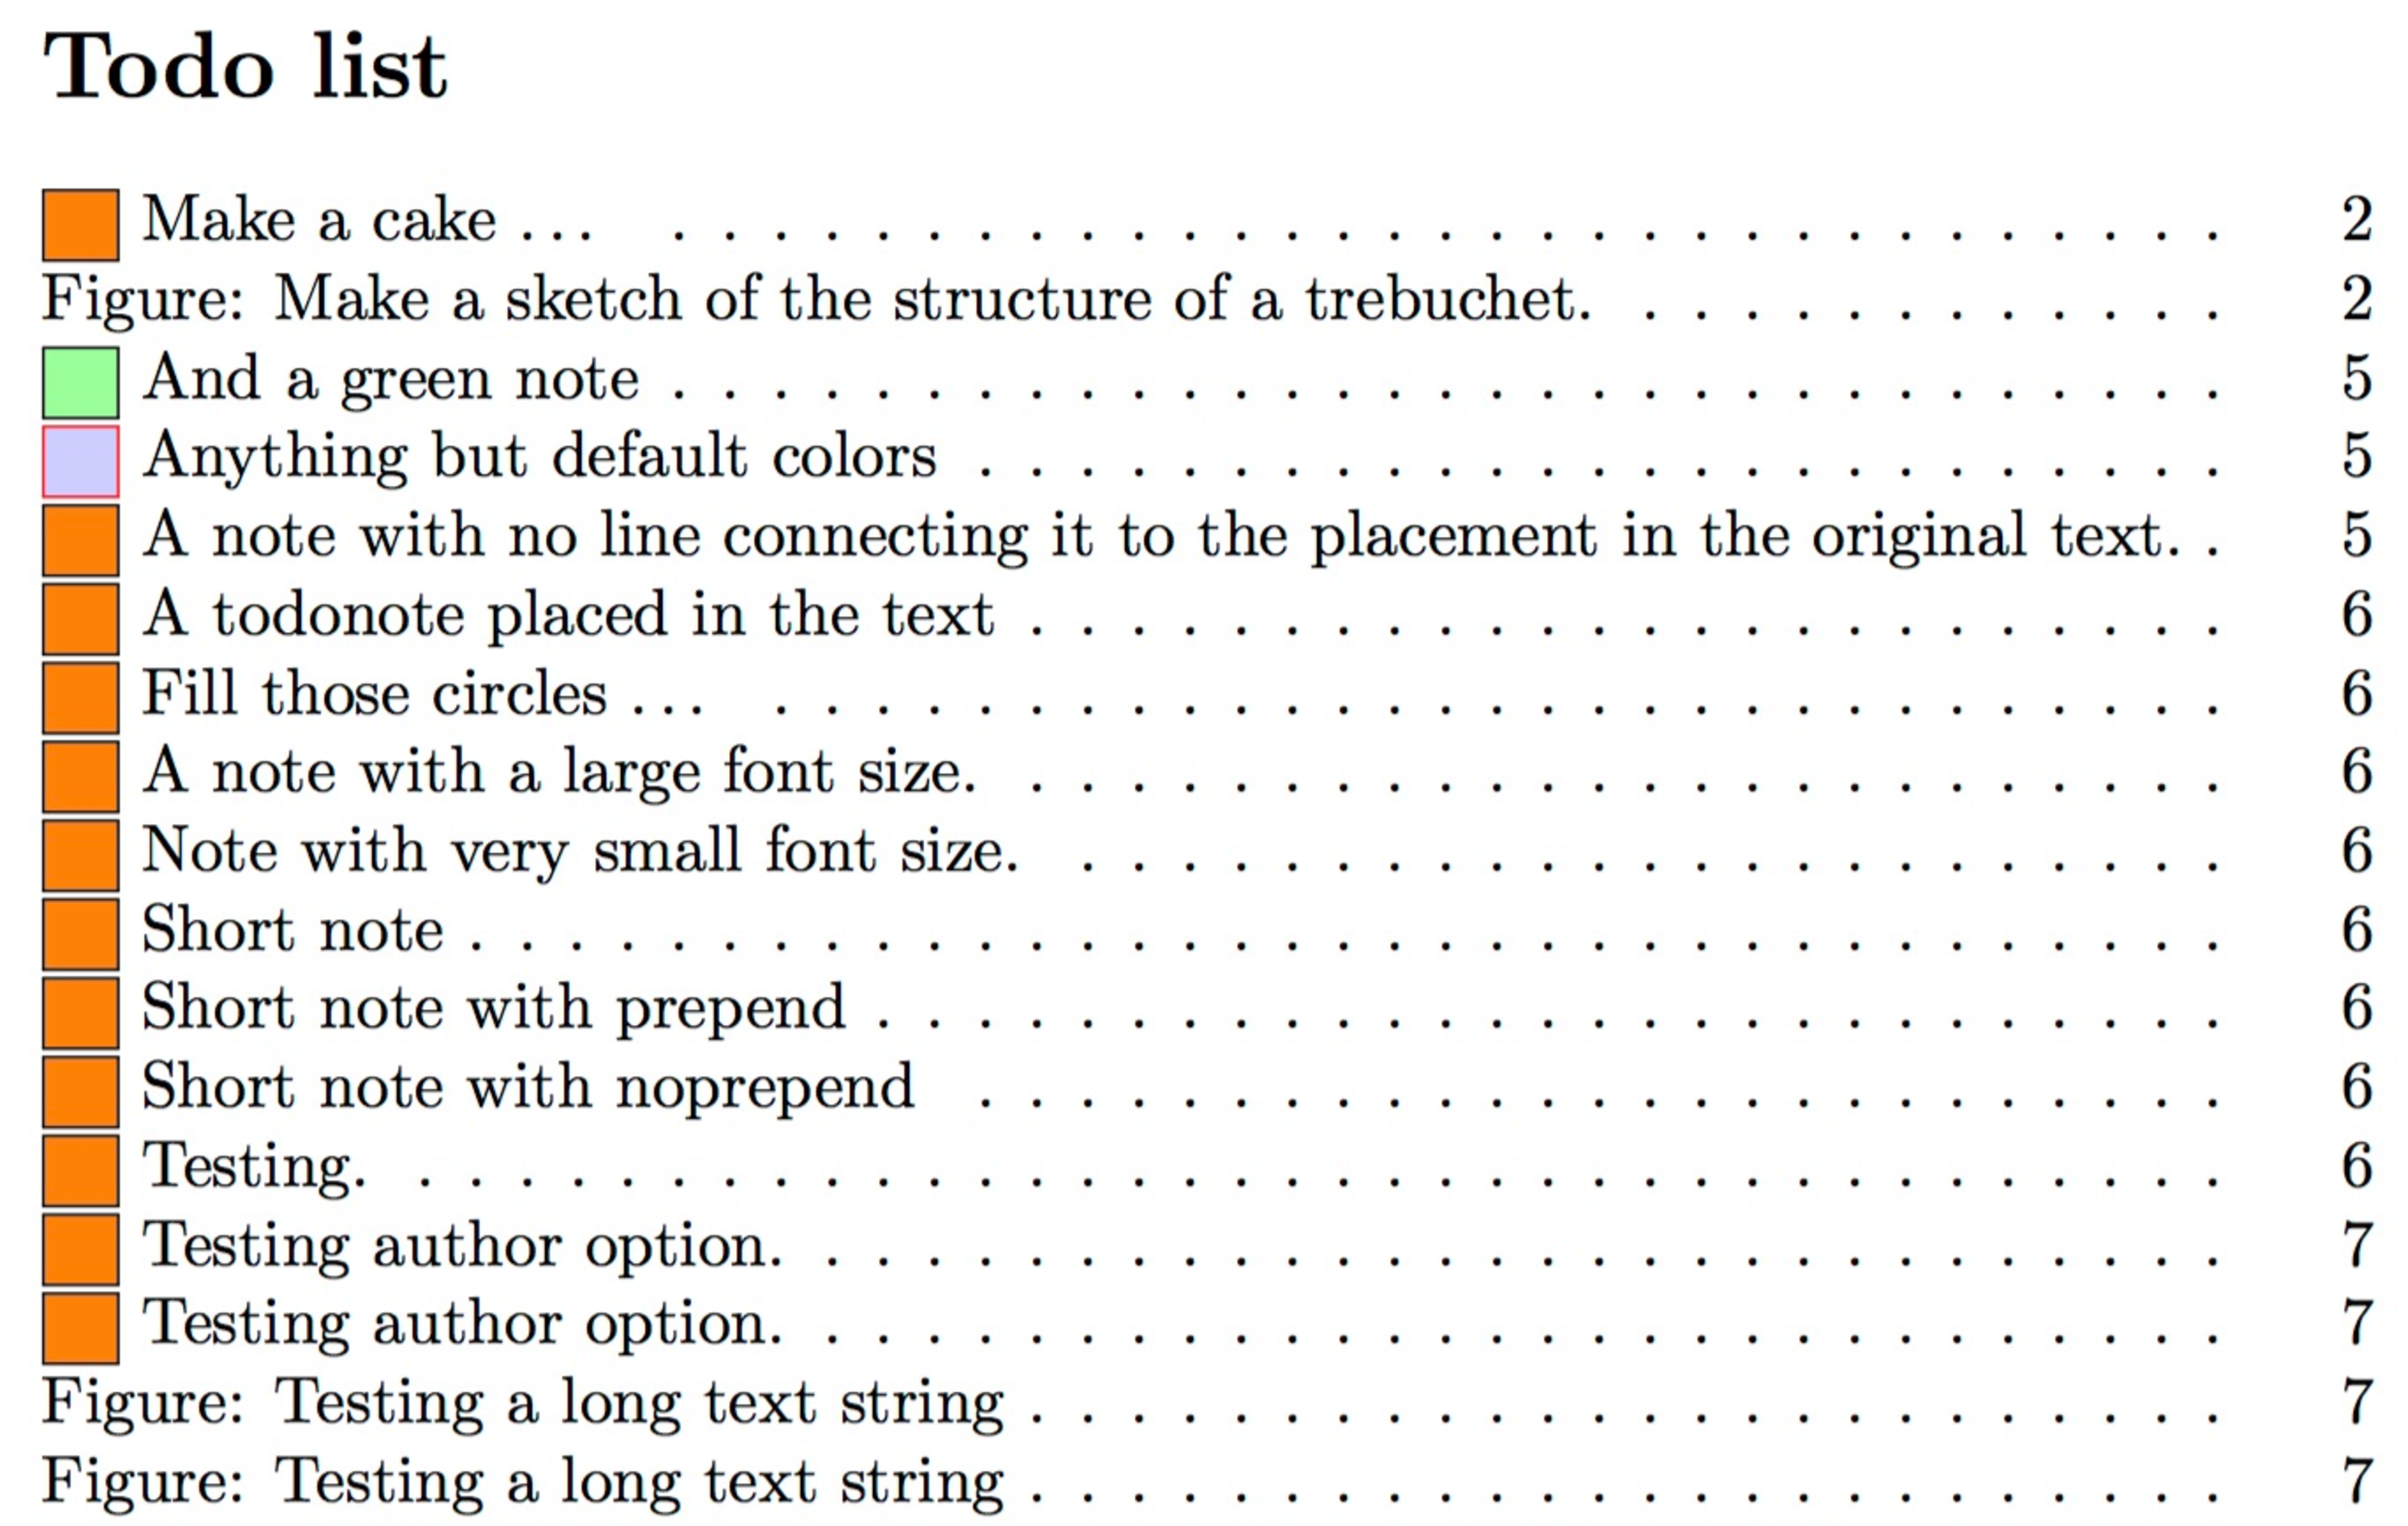
\includegraphics[width=0.9\textwidth]{figures/listoftodos.pdf}
    \end{figure}
    \verb!\listoftodos!
\end{frame}
\begin{frame}[fragile]{Protip zu Todonotes}
    Todos für verschiedene Personen als neue Befehle
    \begin{Verbatim}[frame=single]
\newcommand{\alice}[1]{\todo[color=green!40]{#1}}
\newcommand{\bob}[1]{\todo[color=purple!40]{#1}}
    \end{Verbatim}
    \pause
    \bigskip
    \begin{minipage}{.49\textwidth}
        \begin{Verbatim}[frame=single]
\alice{mach dies}
\bob{mach das}
    \end{Verbatim}
    \end{minipage}
    \begin{minipage}{.49\textwidth}
    \todo[inline, color=green!40]{mach dies}
    \todo[inline, color=purple!40]{mach dies}
    \end{minipage}
    \pause
    \\
    ~\\
    ~\\
    \textit{Beamer} unterstützt nur \verb!inline! todonotes
    \begin{Verbatim}
    \todo[inline]{blablup}
    \end{Verbatim}
    \todo[inline]{blablup}
\end{frame}
\begin{frame}[fragile]{Das cancel Package}
    \begin{Verbatim}
\usepackage{cancel}
\begin{document}
\begin{equation}
    \frac{a\bcancel{b}}{\bcancel{b}}=a
\end{equation}
\end{document}
    \end{Verbatim}
\begin{equation}
    \frac{a\bcancel{b}}{\bcancel{b}}=a
\end{equation}
\pause
\verb!\bcancel{a}! $\bcancel{a}$ \\
\pause
\verb!\cancelto{0}{a}! $\cancelto{0}{a}$ \\
\end{frame}
\begin{frame}[fragile]{Feynman Slash}
    \begin{itemize}
        \item Nicht das cancel Package
        \item \verb!\usepackage{slashed}!
            \pause
        \item \verb!$\gamma^\mu p_\mu = \slashed{p}$!
        \item[$\rightarrow$] $\gamma^\mu p_\mu = \slashed{p} $
    \end{itemize}
    \pause
    \begin{equation}
        (i\slashed{\partial} - m)\psi = 0 
    \end{equation}
\end{frame}
\begin{frame}[fragile]{Das Braket Package}
    \begin{block}{Braket}
        \begin{itemize}
            \item \verb!\usepackage{braket}!
            \item \verb!\bra{a}! $\bra{a}$
            \item \verb!\ket{a}! $\ket{a}$
            \item \verb!\braket{p|x}! $\braket{p|x}$
                \pause
            \item Automatisch angepasste Größe: \verb!Bra!, \verb!Ket!, \dots\\
            \verb!\Braket{ \phi | \frac{\partial^2}{\partial t^2} | \psi }!\\
            $\Braket{ \phi | \frac{\partial^2}{\partial t^2} | \psi }$
        \end{itemize}
    \end{block}
\end{frame}
\begin{frame}{Das \textsc{angekündigte} Microtype Package}
    {\url{ftp://ftp.mpi-sb.mpg.de/pub/tex/mirror/ftp.dante.de/pub/tex/macros/latex/contrib/microtype/microtype.pdf}}
    \begin{block}{Häää}
        \begin{itemize}
            \item \url{http://www.khirevich.com/latex/microtype/} lesenswerte Seite
                \pause
            \item "`Microtype is one of the most notable packages I have ever
                used with LaTeX"'
                \pause
            \item Was macht es?
            \item[$\rightarrow$] Subliminal refinements towards typographical perfection
                \pause
            \item Beispiele von der oben genannten Seite
        \end{itemize}
    \end{block}
\end{frame}
\begin{frame}{Beispiele Microtype}
    \animategraphics[autoplay, loop,width=\linewidth]{1}{figures/microtype-}{0}{1}
    \footnotesize
    von \url{http://www.khirevich.com/latex/microtype/}
\end{frame}
\begin{frame}{Protrusion}
    \begin{quote}
        Glyphs that are small (such as a period) or round (such as the letter
        "o") at the end of a line can be extended beyond the end of the line to
        create a more even line at the edge of the text. This is called
        protrusion, margin kerning, or hanging punctuation\footnote{
        \url{https://en.wikipedia.org/wiki/Microtypography}}
    \end{quote}
\end{frame}
\begin{frame}{Protrusion}
        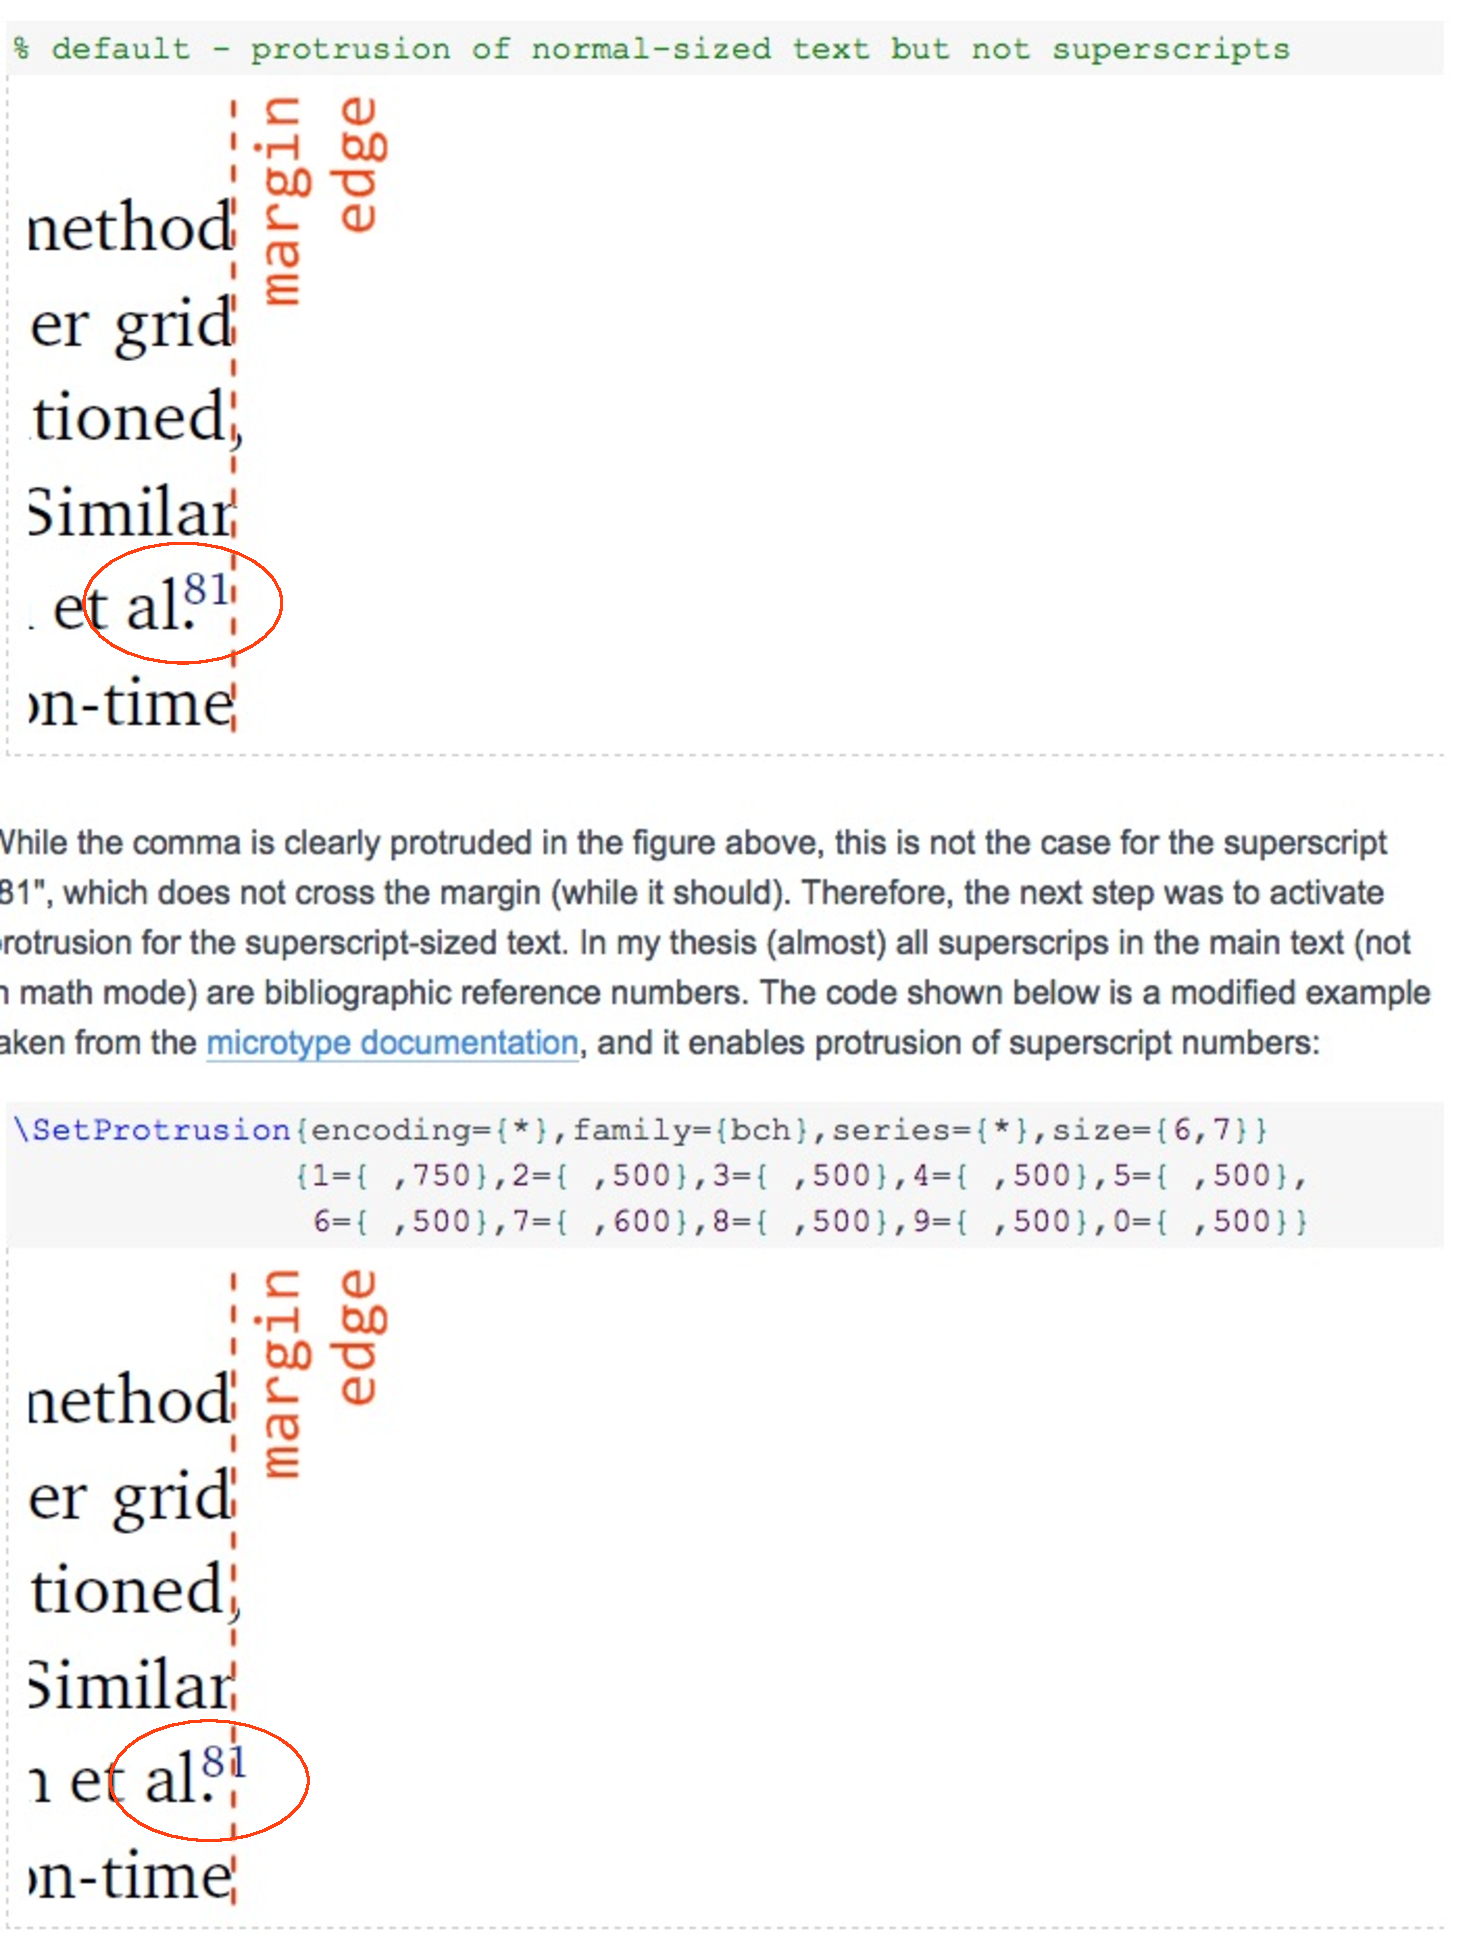
\includegraphics[width=.5\textwidth]{figures/protrusion.pdf}
\end{frame}
\begin{frame}{Microtype Anleitung}
    \animategraphics[autoplay, loop,width=\linewidth]{1}{figures/prot-}{1}{4}
\end{frame}

\begin{frame}[fragile]{Das Anmimate Package}
    \begin{quote}
        A LaTeX package for creating portable, JavaScript driven PDF animations
        from sets of vector graphics or raster image files or from inline
        graphics\footnote{Alexander Grahn \url{http://mirror.unl.edu/ctan/macros/latex/contrib/animate/animate.pdf}}.
    \end{quote}
    \pause
    Also wie gifs, keine wirklichen Videos!
    \pause
    \begin{Verbatim}[fontsize=\small]
\usepackage{animate}
    
\animategraphics[autoplay,loop,width=\linewidth]{1}
    {figures/microtype-}{0}{1}
    \end{Verbatim}
\pause
Geht nur mit \textit{Adobe Reader}
\end{frame}
\begin{frame}[fragile]{Videos - Das media9 Package}{Schon wieder Alexander Grahn,
    muss ein cooler Kerl sein}
    \begin{Verbatim}
\usepackage{media9}
    
\includemedia[<options>]{<poster text>}{
    <main Flash (SWF) file or URL  |  3D (PRC, U3D) file>}
    \end{Verbatim}
    \pause
    \\~\\~\\~\\
    Hää versteh ich nicht!
\end{frame}
\begin{frame}{Wir hören ein Wenig Radio}
    \centering
    \includemedia[
        flashvars={
            source=http://mp3channels.webradio.antenne.de:80/antenne
            &autoPlay=true
        },
        transparent
        ]{\color{blue}\fbox{Listen live to Antenne Bayern}}{%
        APlayer.swf%
}
\end{frame}
    
\begin{frame}{Flugzeug für Tilli}
    \centering
    \includemedia[
        width=7.11cm,height=4cm,
        activate=pageopen,
        flashvars={
            modestbranding=1 % no YT logo in control bar
            &autohide=1 % controlbar autohide
            &showinfo=0 % no title and other info before start
            &rel=0 % no related videos after end
        },
        url % Flash loaded from URL
    ]{}{http://www.youtube.com/v/bHub7MwGJjE?rel=0}
\end{frame}
\begin{frame}[fragile]{Code für Video}
    \begin{Verbatim}[frame=single]
\includemedia[
    width=7.11cm,height=4cm,
    activate=pageopen,
    flashvars={
        modestbranding=1 % no YT logo in control bar
        &autohide=1 % controlbar autohide
        &showinfo=0 % no title and other info before start
        &rel=0 % no related videos after end
    },
    url % Flash loaded from URL
]{}{http://www.youtube.com/v/bHub7MwGJjE?rel=0}
    \end{Verbatim}
    \pause
    Zur Url: \\
        \begin{itemize}
            \item Auf Youtube: \url{https://www.youtube.com/watch?v=bHub7MwGJjE}
            \item Nehme Teil nach \verb!v=!
        \item \verb!]{}{http://www.youtube.com/v/bHub7MwGJjE?rel=0}!
    \end{itemize}
\end{frame}
\begin{frame}[t]
    \begin{block}{Hier eine interne Videodatei}
        \centering
    \includemedia[
        label=MeinFilm,
        width=0.6\linewidth,height=0.45\linewidth,
        addresource=flugzeug.mp4, %two video files
%addresource=Film2.avi,
        transparent, %transparent player background
        activate=pageopen,
        flashvars={source=flugzeug.mp4
            &hideBar=false
            &loop=true % loop video
            &controlBarMode=floating
            &controlBarAutoHide=false
            &scaleMode=letterbox % preserve aspect ratio while scaling the video
        }
    ]{}{VPlayer.swf} \par
    \mediabutton[
        mediacommand=MeinFilm:playPause,
        overface=\color{blue}{\fbox{\strut Play/Pause}},
        downface=\color{red}{\fbox{\strut Play/Pause}}
    ]{\fbox{\strut Play/Pause}}{Flugzeug.mp4}
\end{block}
\end{frame}
\begin{frame}[fragile]{Lokales Video - mp4}{Video muss H.264 encoded sein, container mp4}
    \begin{Verbatim}[frame=single]
\includemedia[
    label=some_dice,
    width=0.4\linewidth,height=0.3\linewidth,
    activate=pageopen,
    addresource=random.mp4,
    flashvars={
        source=random.mp4
        &loop=true           % loop video
        &scaleMode=letterbox % preserve aspect ratio 
                             % while scaling the video
    }
]{}{VPlayer.swf}             % used video player
    \end{Verbatim}
    Ansonsten: Anleitung lesen!
\end{frame}

%\begin{frame}
  %\frametitle{Youtube video}
  %\includemedia[
%width=7.11cm,height=4cm,
%activate=pageopen,
%flashvars={
%modestbranding=1 % no YT logo in control bar
%&autohide=1 % controlbar autohide
%&showinfo=0 % no title and other info before start
%&rel=0 % no related videos after end
%},
%url % Flash loaded from URL
%]{}{http://www.youtube.com/v/9bZkp7q19f0?rel=0}
%\end{frame}

\end{document}

\begin{frame}{}
    \begin{block}{}
        \begin{itemize}
            \item 
        \end{itemize}
    \end{block}
\end{frame}

